\documentclass[letterpaper,12pt]{article}

\usepackage{threeparttable}
\usepackage{geometry}
\geometry{letterpaper,tmargin=1in,bmargin=1in,lmargin=1.25in,rmargin=1.25in}
\usepackage[format=hang,font=normalsize,labelfont=bf]{caption}
\usepackage{amsmath}
\usepackage{multirow}
\usepackage{array}
\usepackage{delarray}
\usepackage{amssymb}
\usepackage{amsthm}
\usepackage{listings}
\usepackage{lscape}
\usepackage{natbib}
\usepackage{setspace}
\usepackage{float,color}
\usepackage[pdftex]{graphicx}
\usepackage{pdfsync}
\usepackage{verbatim}
\usepackage{placeins}
\usepackage{mathrsfs}  
\usepackage{geometry}
\usepackage{pdflscape}
\graphicspath{ {images/} }
\synctex=1
\usepackage{hyperref}
\hypersetup{colorlinks,linkcolor=red,urlcolor=blue,citecolor=red}
\usepackage{bm}
\theoremstyle{definition}
\newtheorem{theorem}{Theorem}
\newtheorem{acknowledgement}[theorem]{Acknowledgement}
\newtheorem{algorithm}[theorem]{Algorithm}
\newtheorem{axiom}[theorem]{Axiom}
\newtheorem{case}[theorem]{Case}
\newtheorem{claim}[theorem]{Claim}
\newtheorem{conclusion}[theorem]{Conclusion}
\newtheorem{condition}[theorem]{Condition}
\newtheorem{conjecture}[theorem]{Conjecture}
\newtheorem{corollary}[theorem]{Corollary}
\newtheorem{criterion}[theorem]{Criterion}
\newtheorem{definition}{Definition} % Number definitions on their own
\newtheorem{derivation}{Derivation} % Number derivations on their own
\newtheorem{example}[theorem]{Example}
\newtheorem{exercise}[theorem]{Exercise}
\newtheorem{lemma}[theorem]{Lemma}
\newtheorem{notation}[theorem]{Notation}
\newtheorem{problem}[theorem]{Problem}
\newtheorem{proposition}{Proposition} % Number propositions on their own
\newtheorem{remark}[theorem]{Remark}
\newtheorem{solution}[theorem]{Solution}
\newtheorem{summary}[theorem]{Summary}
\bibliographystyle{aer}
\newcommand\ve{\varepsilon}
\renewcommand\theenumi{\roman{enumi}}
\newcommand\norm[1]{\left\lVert#1\right\rVert}

\begin{document}


\subsection*{12.1}


 mean($Y_t$) =  0.478790919848\\
 mean($c_t$)=  0.289053260303\\
 var($Y_t$) =  0.000118971936416\\
 var($c_t$) =  4.33619219953e-05\\
 corr($k_t,Y_t$) =  0.770254601008\\
 corr($k_t,k_{t+1}$) =  0.776769702307\\

Parameters are as follows:
\[\alpha =  0.414999996868\]
\[\beta =  0.954849795539\]
\[\rho =  0.596119118343\]
\[\mu =  -0.0469562926534\]
\[\sigma =  0.0137100107631\]


Computation time = 93.0396201611 seconds.\\
\\
Criterion functional value = $3.55 \times 10^{-5}$
\\

Included moments: 
\[\begin{tabular}{rrrrrr}
\hline
mean(Y_t) &   mean(c_t) &     var(Y_t) &     var(c_t) &   corr(k_t,Y_t) &   corr(k_t,k_{t+1}) \\
\hline
   0.478754 &   0.289042 & 0.000118968 & 4.33636e-05 &      0.773421 &        0.773421 \\
   0.478791 &   0.289053 & 0.000118972 & 4.33619e-05 &      0.770255 &        0.77677  \\
\hline
\end{tabular}\]
Outside moments:
\[\begin{tabular}{rrrrr}
\hline
mean(k_t) &     var(k_t) &   corr(k_t,c_t) &   corr(y_t,c_t) &   corr(c_t,c_{t+1}) \\
\hline
   0.189713 & 1.84274e-05 &      0.773421 &             1 &        0.773061 \\
   0.18977  & 1.89667e-05 &      0.770255 &             1 &        0.763796 \\
\hline
\end{tabular}\]



\subsection*{14.1}


\noindent mean = 720.277975327\\
median =  172.21\\
max =  227967.25\\
min =  0.01\\
standard deviation =  3972.66375639

\begin{figure}[htb]\centering \captionsetup{width=4.0in}
        \caption{\label{Histogram<800}\textbf{Histogram }}
        \fbox{\resizebox{3.0in}{2.0in}{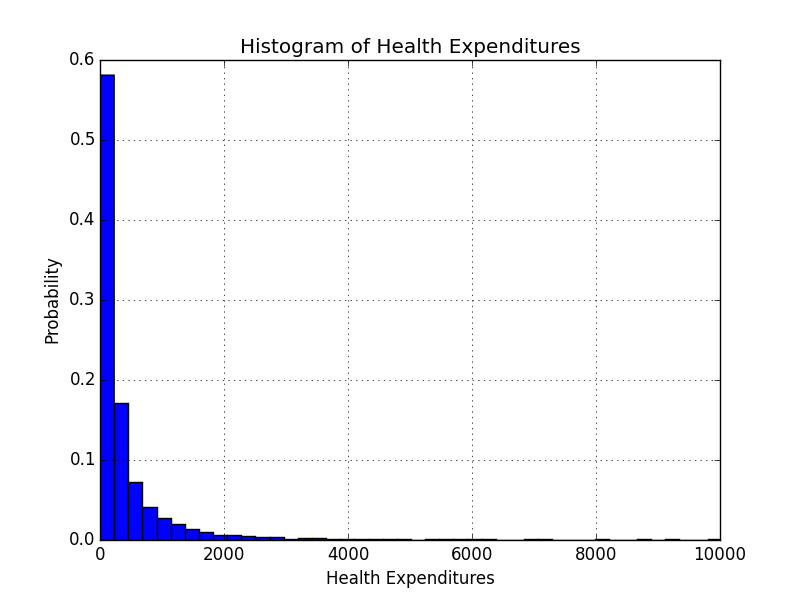
\includegraphics{histogramone.png}}}
\end{figure}



\begin{figure}[htb]\centering \captionsetup{width=4.0in}
        \caption{\label{Histogram<800}\textbf{Histogram}}
        \fbox{\resizebox{3.0in}{2.0in}{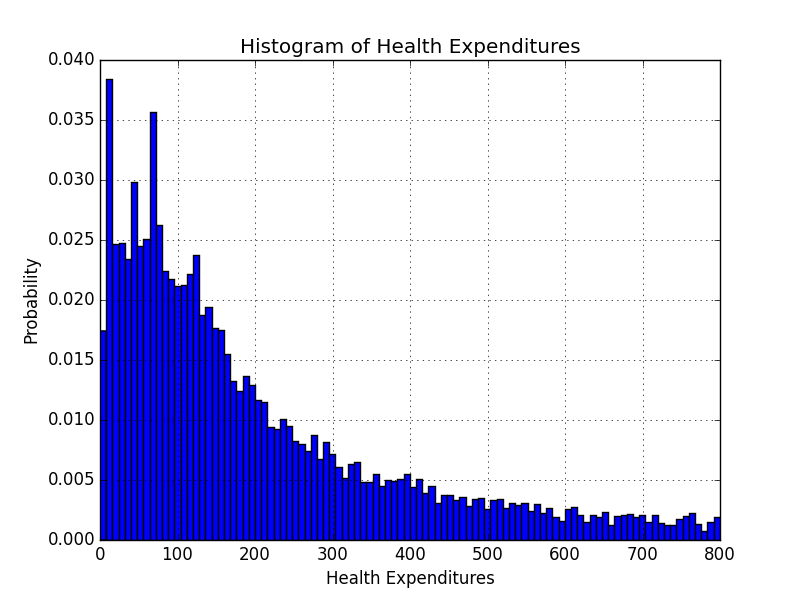
\includegraphics{fourteenoneii.png}}}
\end{figure}
Data is skewed in second graph, so we see the more relevant part of the data. For this reason it might be preferred.


\subsection*{14.2}


\[\hat{\alpha} =  0.472506084871\]
\[\hat{\beta} =  1524.4132857\]
\[ \text{Value of maximized log likelihood function} = -77723.4734271\]

\begin{figure}[htb]\centering \captionsetup{width=4.0in}  
        \caption{\label{Histogram<800}\textbf{Histogram with $\gamma$ distribution}}
        \fbox{\resizebox{4.0in}{3.0in}{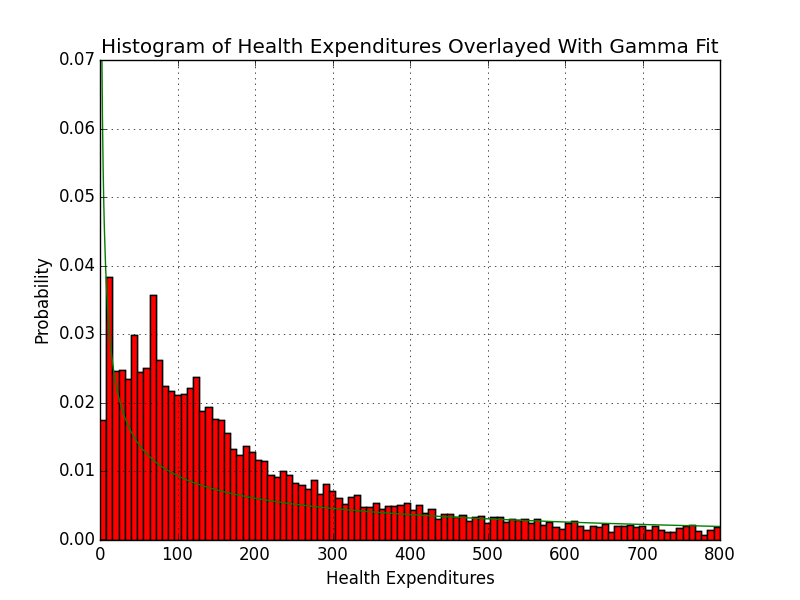
\includegraphics{fourteentwo.png}}}
\end{figure}

\newpage



\subsection*{14.3}


\begin{figure}[htb]\centering \captionsetup{width=4.0in}
        \caption{\label{Histogram<800}\textbf{Histogram fitted with generalized $\gamma$}}
        \fbox{\resizebox{4.0in}{3.0in}{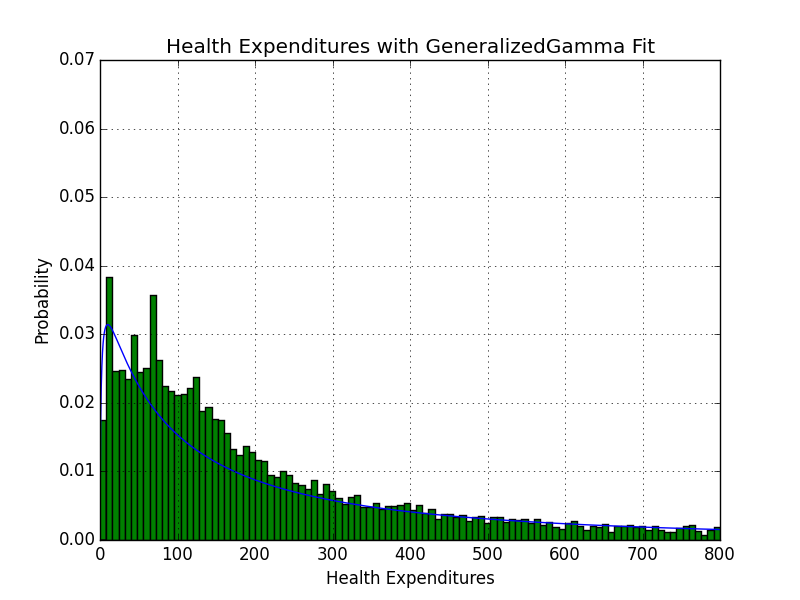
\includegraphics{fourteenthree.png}}}
\end{figure}

We got the estimated values 
\[\hat{\alpha}=2.15224965\]
\[\hat{\beta}=0.00205435987\]
\[\hat{m}=0.202900153\]
\[\text{Value of the maximized log likelihood function} = 75047:640676131472\]
\subsection*{14.4}


\noindent \[\text{Log likelihood} =  -74892.9454288\]
\[\hat{a} =  0.0986012857732\]
\[\hat{b} =  13299499492.2\]
\[\hat{p} =  52.1244834389\]
\[\hat{q} =  307.688083445\]

\begin{figure}[htb]\centering \captionsetup{width=4.0in}
        \caption{\label{Histogram<800}\textbf{Histogram fitted with generalized $\beta$ GB2}}
        \fbox{\resizebox{3.0in}{2.0in}{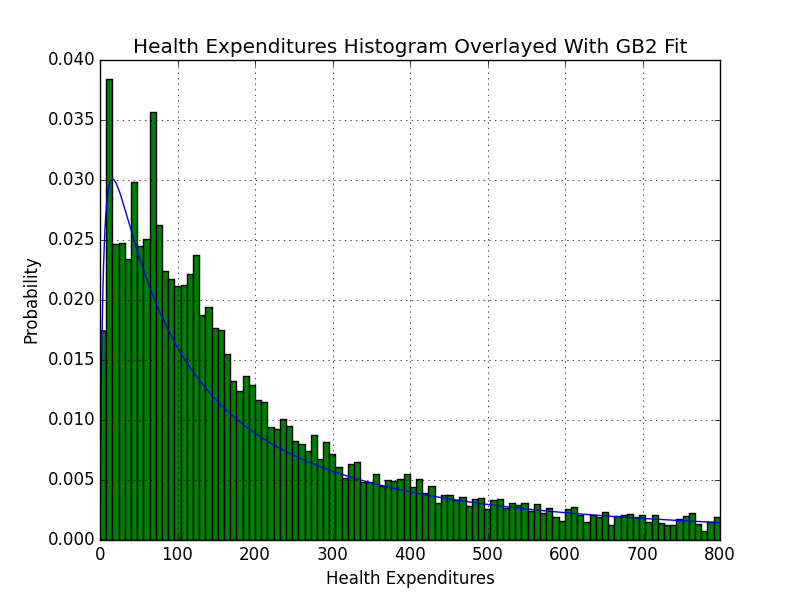
\includegraphics{fourteenfour.png}}}
\end{figure}


\subsection*{14.5}


\begin{figure}[htb]\centering \captionsetup{width=4.0in}
        \caption{\label{Histogram<800}\textbf{Histogram fitted with GA, GG and GB2 distributions}}
        \fbox{\resizebox{4.0in}{3.0in}{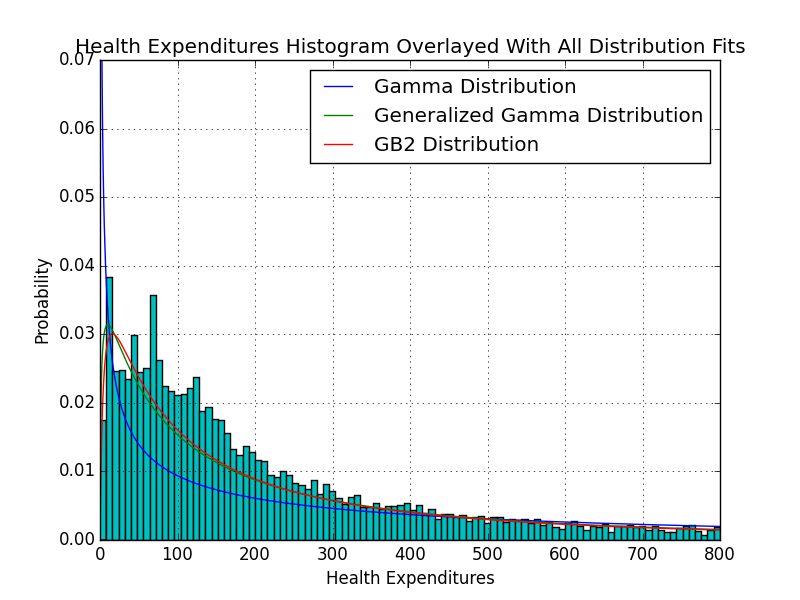
\includegraphics{fourteenfive.png}}}
\end{figure}

The GB2 appears to have the best fit, but the likelihood ratio test will give us a surefire way to tell. We have that\\
Gamma likelihood:  -77723.4734271\\
Generalized Gamma likelihood:  -75042.2927752\\
GB2 likelihood:  -74892.9454288\\
\[ \implies \text{GB2 has best fit}\]


\subsection*{14.6}



\begin{figure}[htb]\centering \captionsetup{width=4.0in}
        \caption{\label{Histogram<800}\textbf{Histogram with income distribution}}
        \fbox{\resizebox{4.0in}{3.0in}{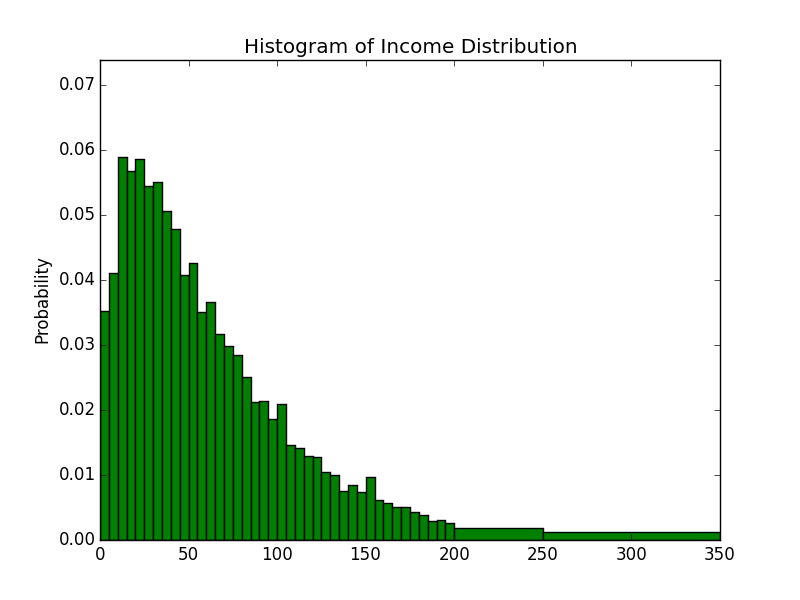
\includegraphics{fourteensix.png}}}
\end{figure}

\subsection*{14.7}


\[\hat \mu= 3.97691922\]
\[\hat \sigma=1.0466081\] 
\[ \text{Value of the miminized criterion function} = 0.000042503325515859232.\]

\begin{figure}[htb]\centering \captionsetup{width=4.0in}
        \caption{\label{Histogram<800}\textbf{Histogram with income distribution with lognormal fit}}
        \fbox{\resizebox{4.0in}{3.0in}{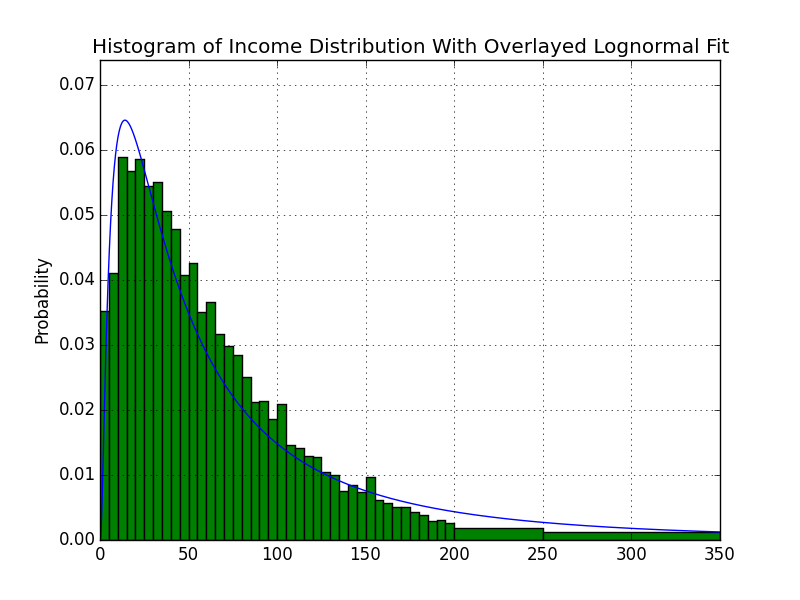
\includegraphics{fourteenseven.png}}}
\end{figure}

\subsection*{14.8}


\[\hat \alpha= 1.43059137\]
\[\hat \beta= 44.43445121\]
\[\text{Value  of  the  miminized  criiterion  function}=0.00000066226533019988027\]
\begin{figure}[htb]\centering \captionsetup{width=4.0in}
        \caption{\label{Histogram<800}\textbf{Histogram with income distribution with $\gamma$ distributional fit}}
        \fbox{\resizebox{4.0in}{3.0in}{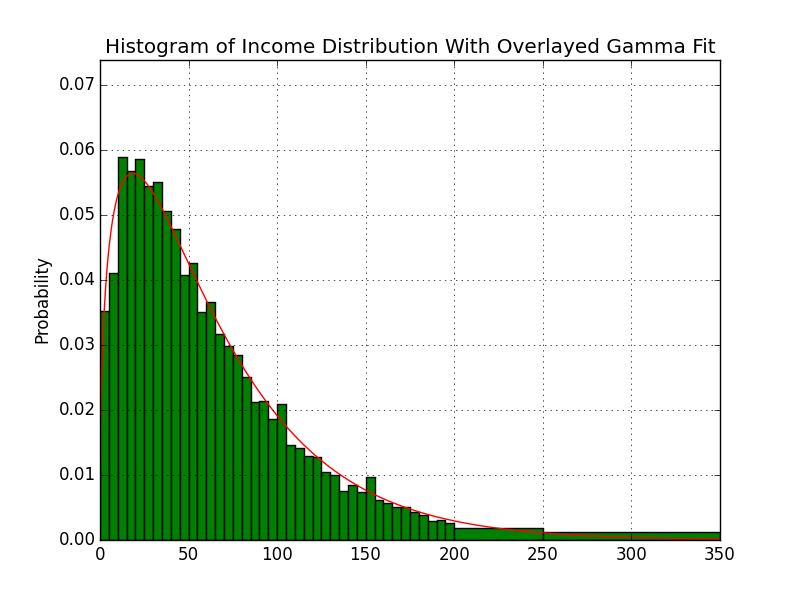
\includegraphics{fourteeneight.png}}}
\end{figure}
\newpage


\subsection*{14.9}



\begin{figure}[htb]\centering \captionsetup{width=4.0in}
        \caption{\label{Histogram<800}\textbf{Histogram with income distribution with both distributions}}
        \fbox{\resizebox{4.0in}{3.0in}{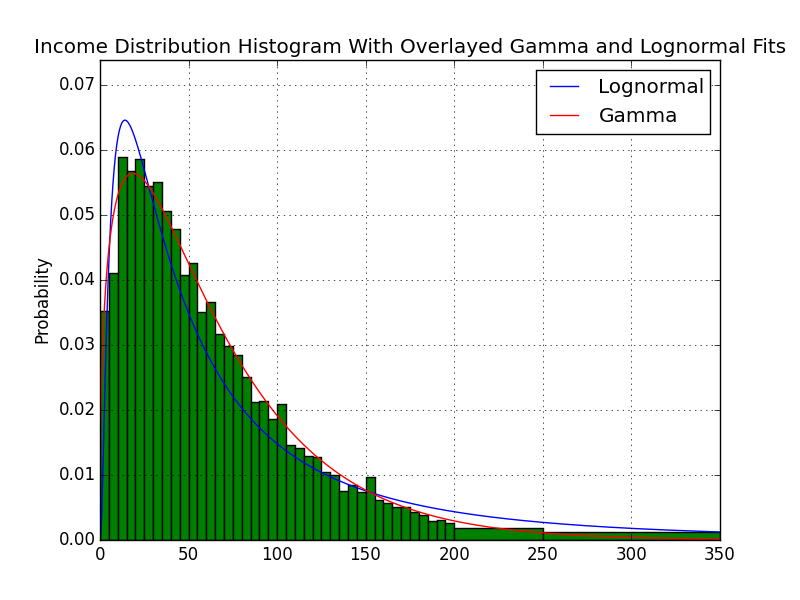
\includegraphics{fourteennine.png}}}
\end{figure}

By examining the following values we can determine which is a more precise fit\\
\[\text{Log-normal mean} =  99641.2728153\]
\[\text{Log-normal median} =  51901.0294037\]
\[\text{Gamma mean} =  65008.2095102\]
\[\text{Gamma median} =  50218.0027898\]
\[\text{Empirical mean} =  69677\]
\[\text{Empirical median} =  50504\]

Gamma more closely resembles empirical and thus we have that it is the most precise fit.



\end{document}
